\providecommand{\main}{../../../..}
\documentclass[\main/dresen_thesis.tex]{subfiles}
\begin{document}
  \label{sec:colloidalCrystals:layers:pnr}

  \begin{figure}[tb]
    \centering
    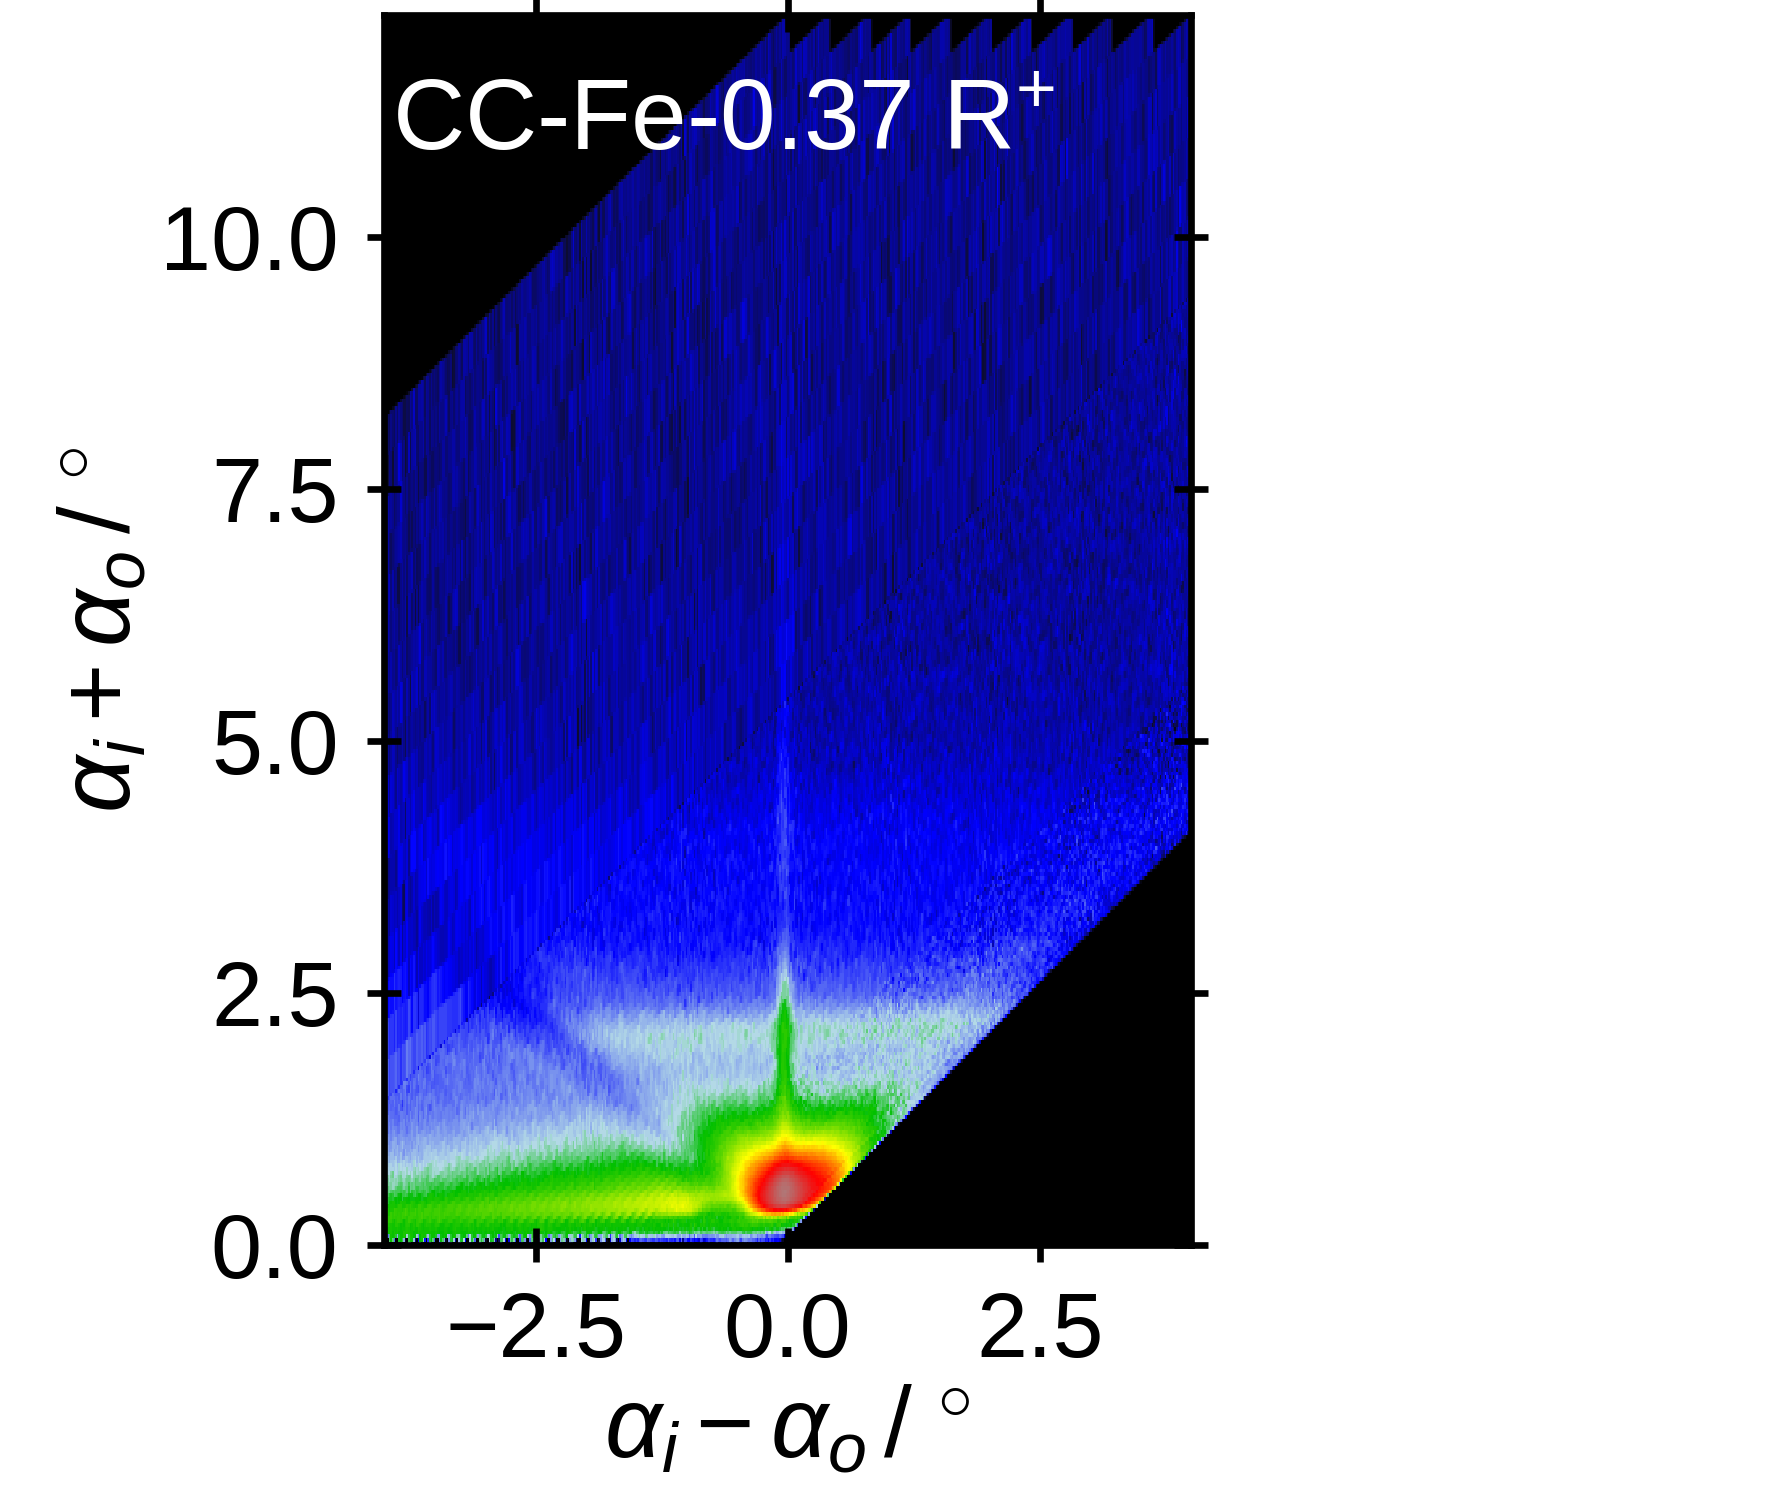
\includegraphics{colloidalCrystals_PNR_CC_Fe_0_37_rem_ud_ReflectivityMapFC}
    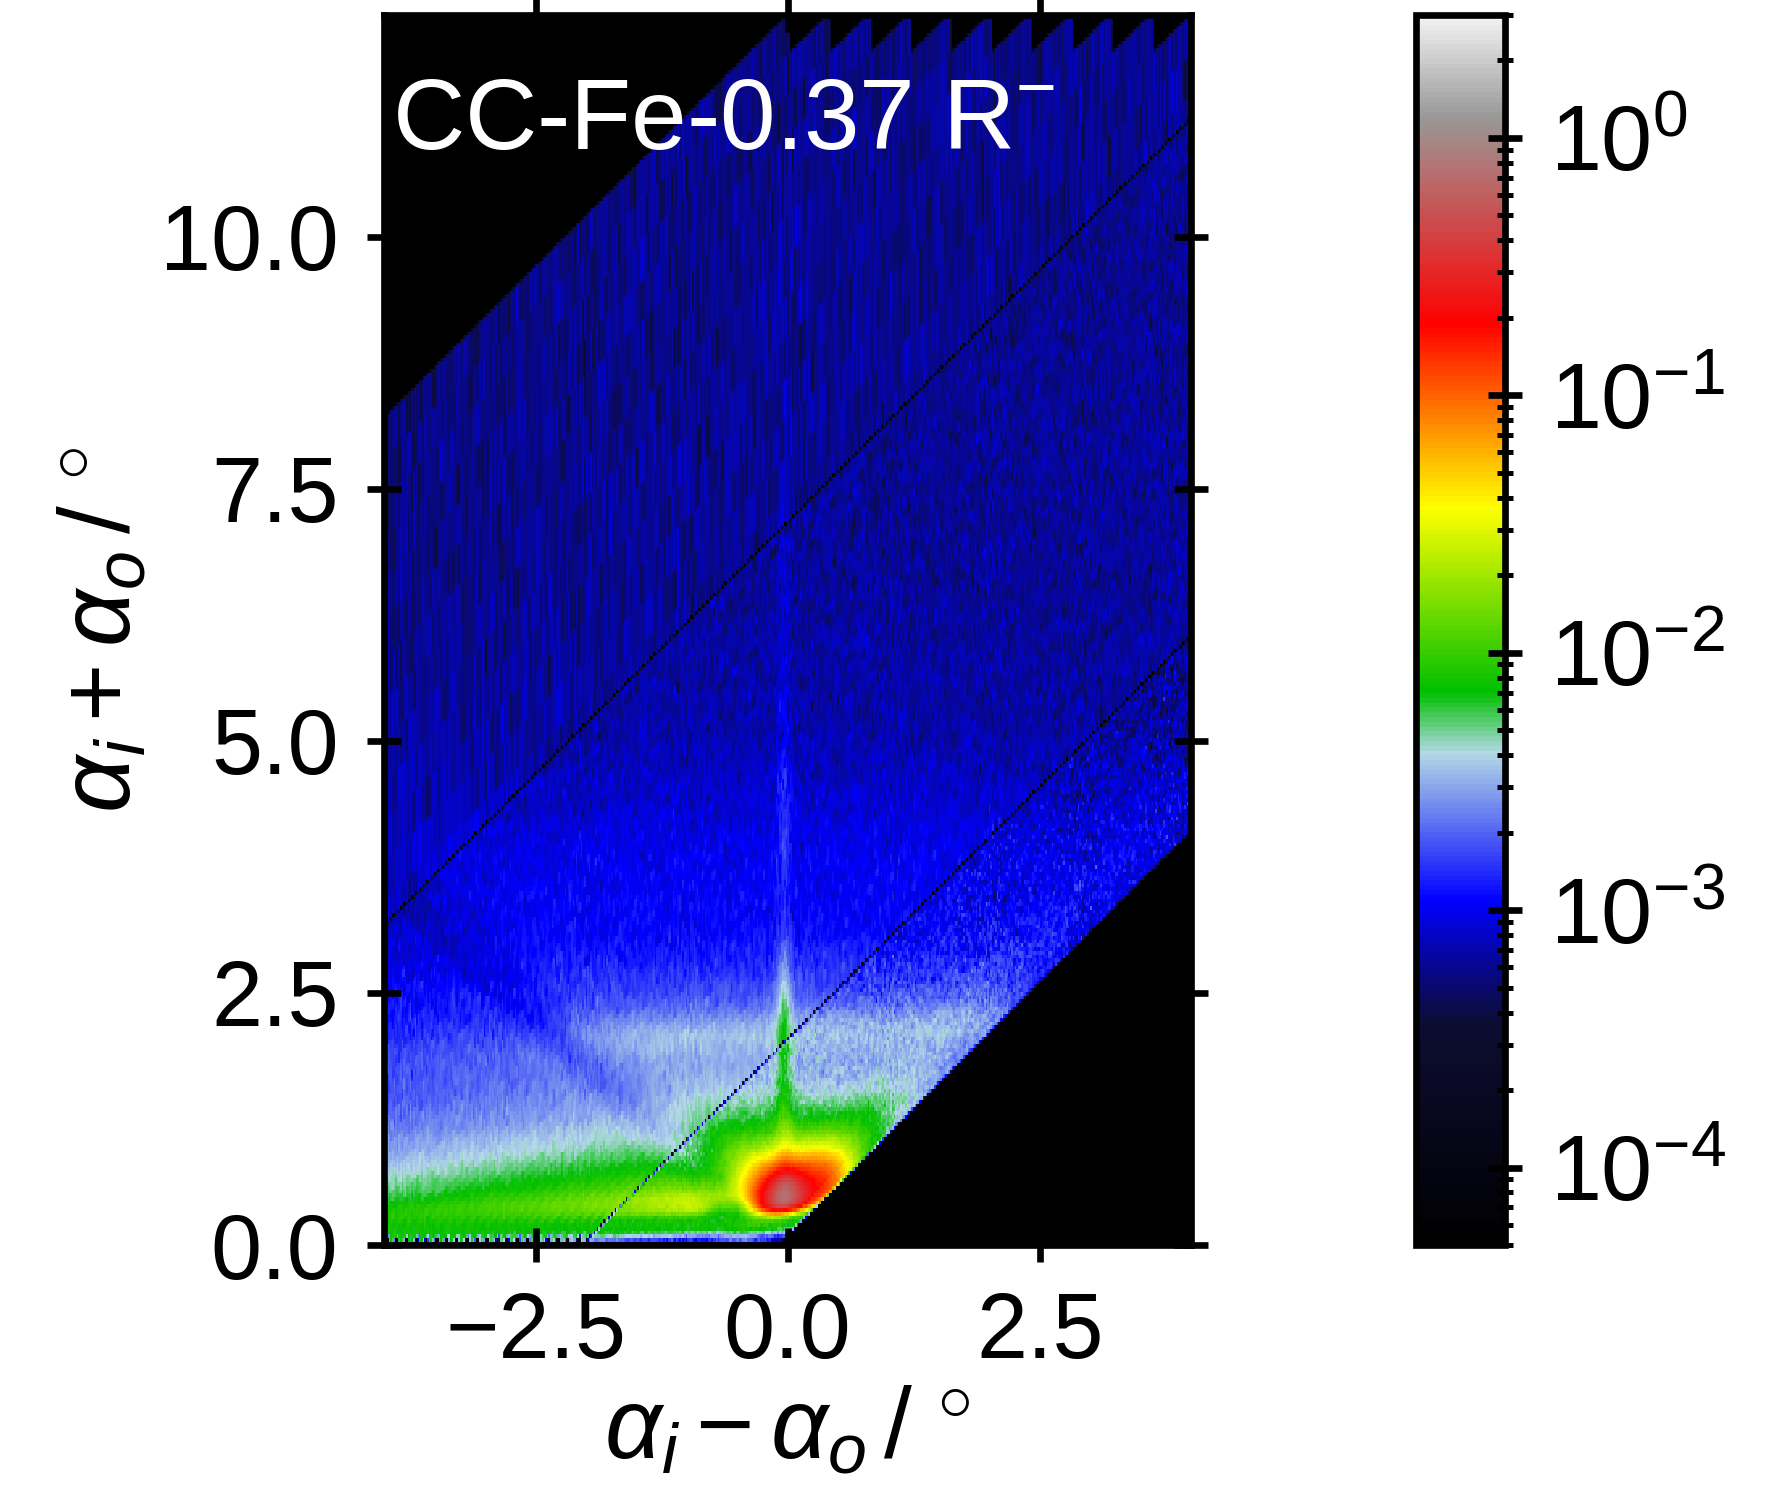
\includegraphics{colloidalCrystals_PNR_CC_Fe_0_37_rem_dd_ReflectivityMapFC}
    \caption{\label{fig:colloidalCrystals:pnr} CC-Fe-0.37 FC Remanence Maps}
  \end{figure}
  % \begin{table}[!htbp]
  %   \centering
  %   \caption{\label{tab:looselyPackedNP:nanoparticle:gisaxs}Parameters for the hard-sphere structure factor in Percus-Yervick approximation shown in \reffig{fig:looselyPackedNP:layer:gisaxs} for both SC-IOS-11 and SC-IOS-7. $R_\mathrm{HS}$ is the hard-sphere radius and $\eta$ the packing fraction of the structure factor.}
  %   \begin{tabular}{ c | l | l }
  %     \rule{0pt}{2ex} \textbf{GISAXS}  & \textbf{SC-IOS-11} & \textbf{SC-IOS-7} \\
  %     \hline
  %     \rule{0pt}{2ex} $R_\mathrm{HS} \, / \unit{nm}$          & $5.655(2)$           & $3.872(4)$\\
  %     \rule{0pt}{2ex} $\eta          \, / \unit{\%}$          & $43.88(3)$           & $34.20(9)$\\
  %     \hline
  %   \end{tabular}
  % \end{table}


  \begin{figure}[tb]
    \centering
    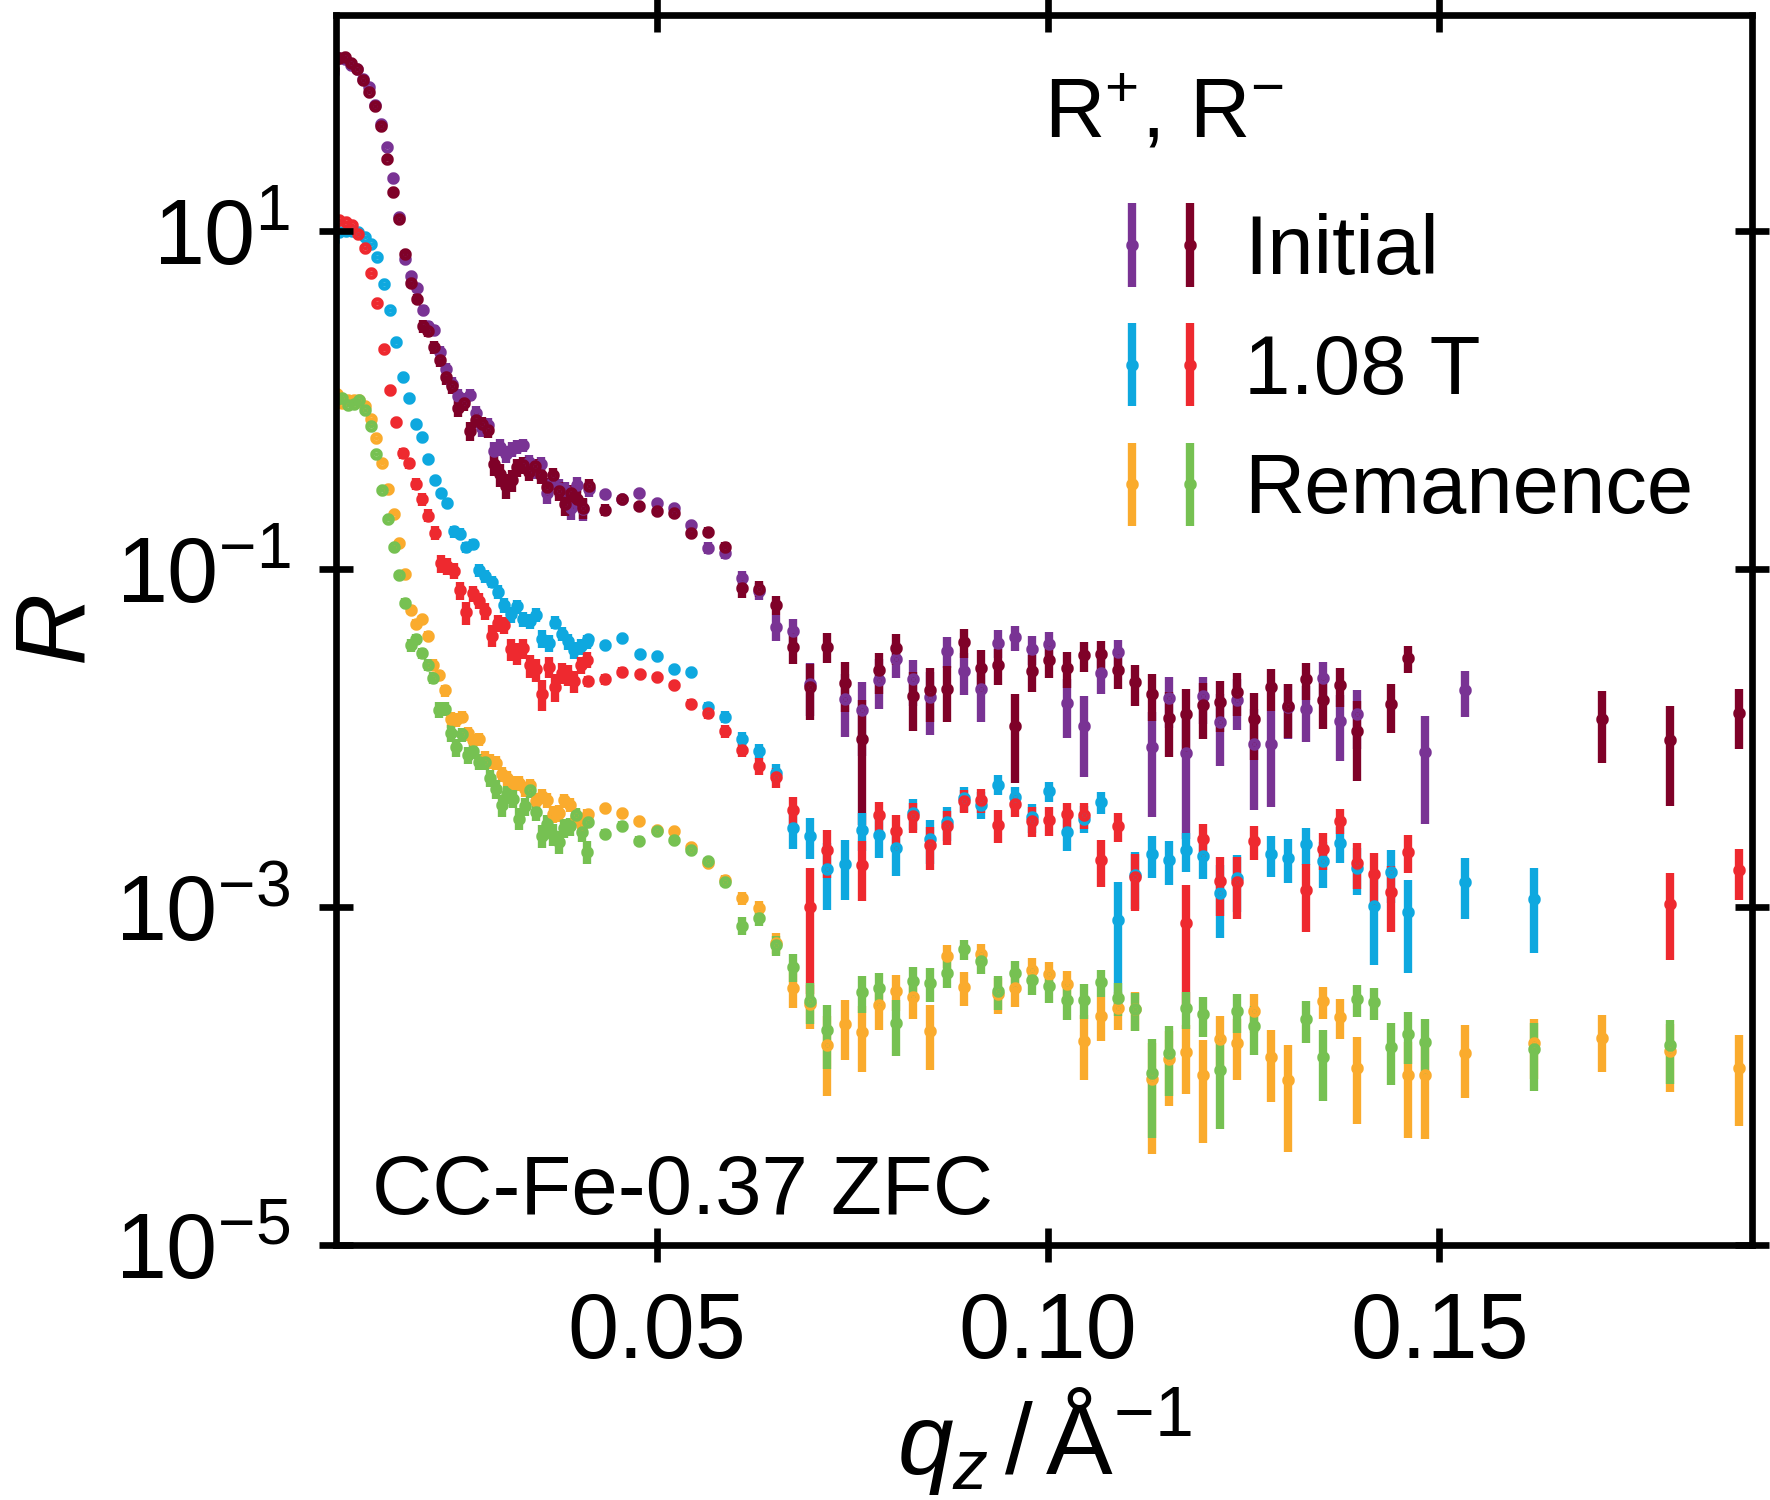
\includegraphics{colloidalCrystals_VerticalStructure_CC-Fe-0_37_PNR_ZFC10K}
    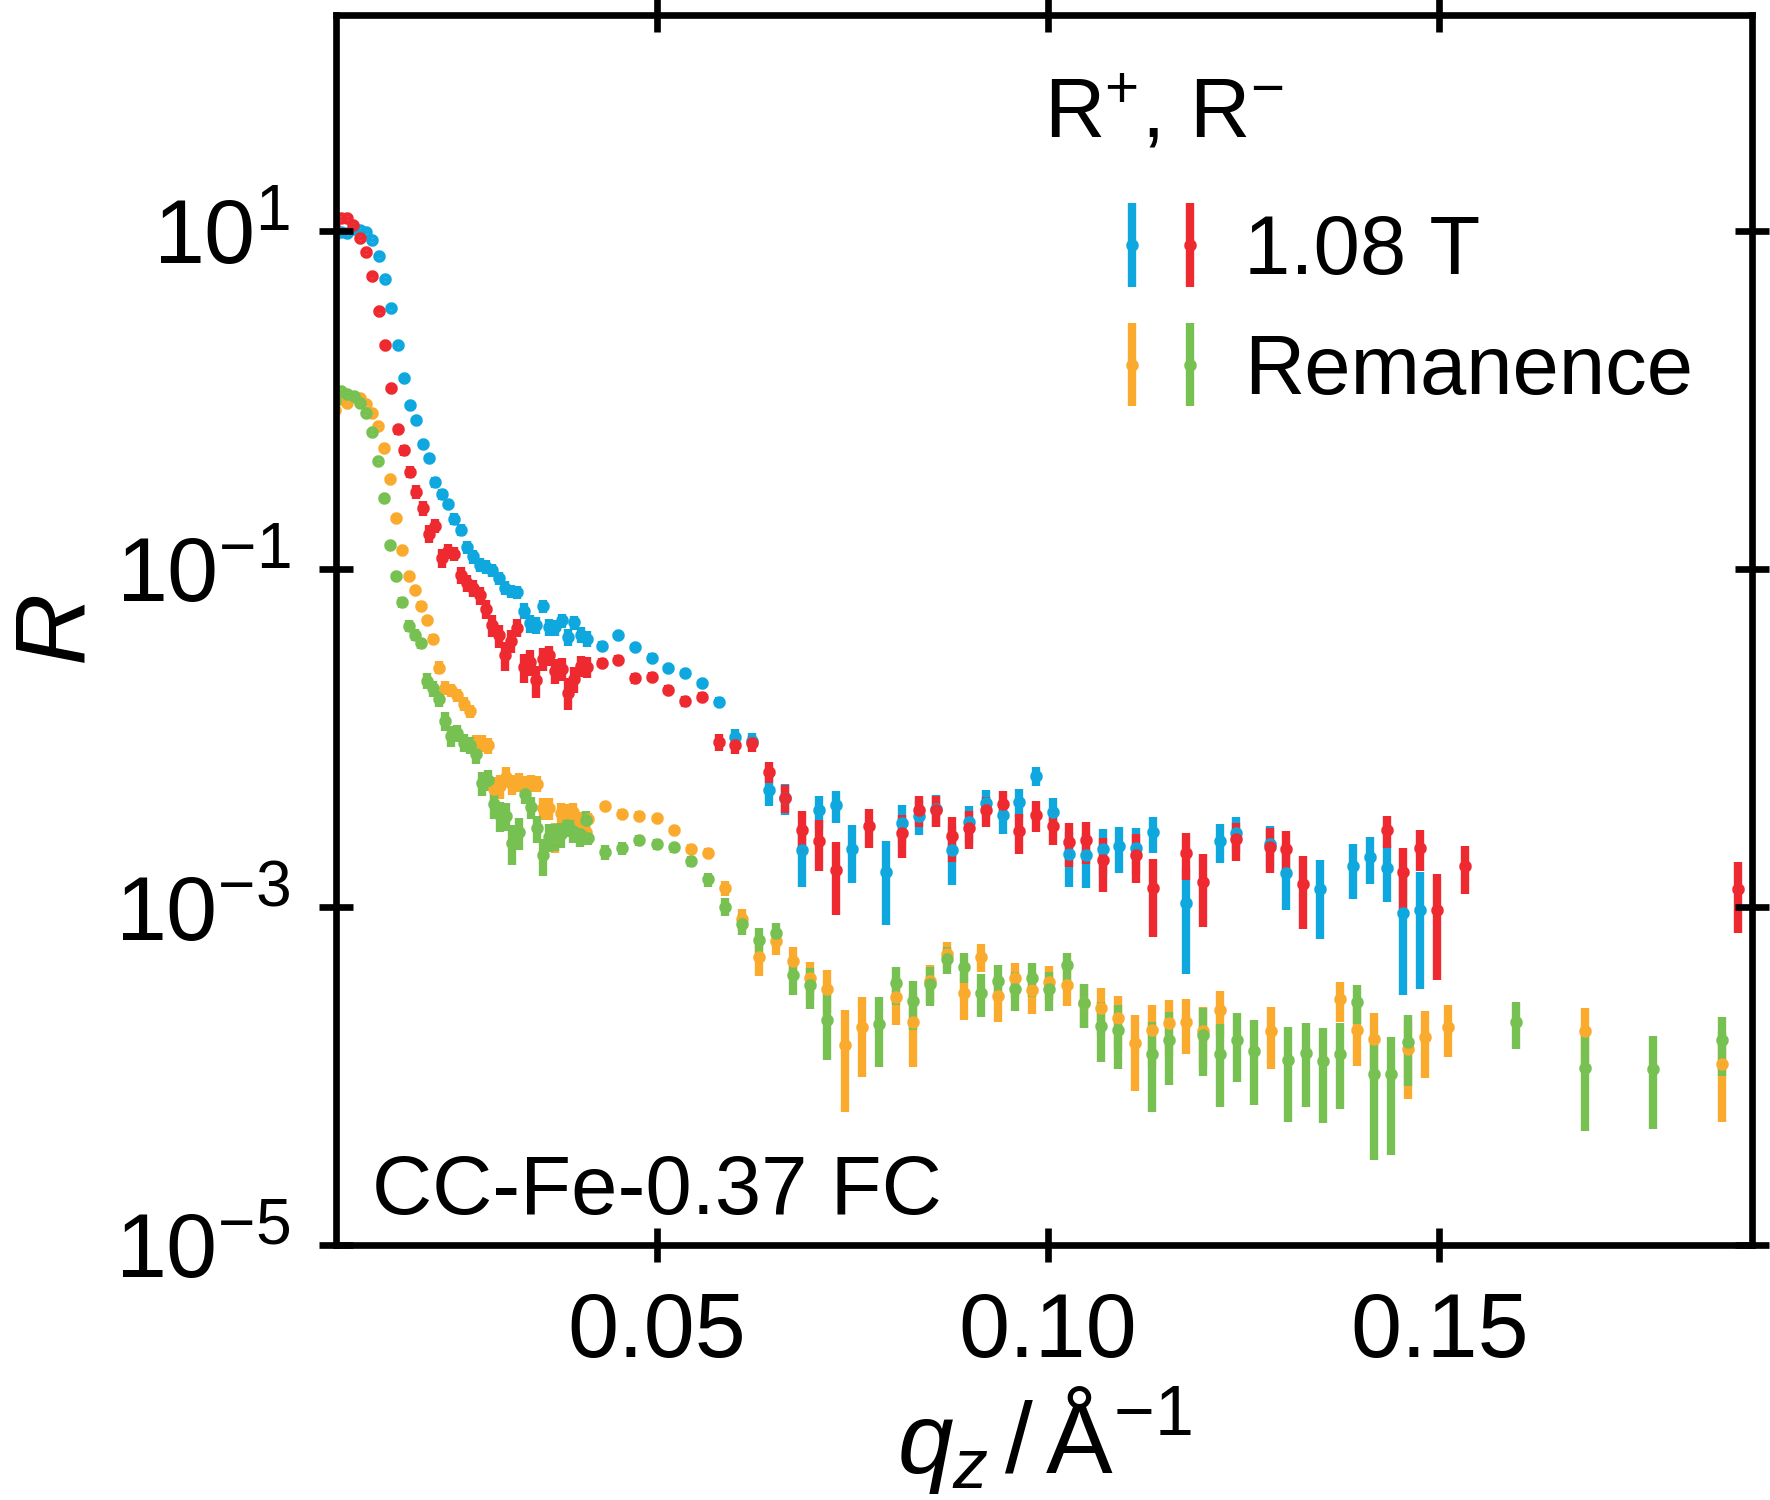
\includegraphics{colloidalCrystals_VerticalStructure_CC-Fe-0_37_PNR_FC10K}
    \caption{\label{fig:colloidalCrystals:pnr} CC-Fe-0.37 ZFC and FC}
  \end{figure}

  \begin{figure}[tb]
    \centering
    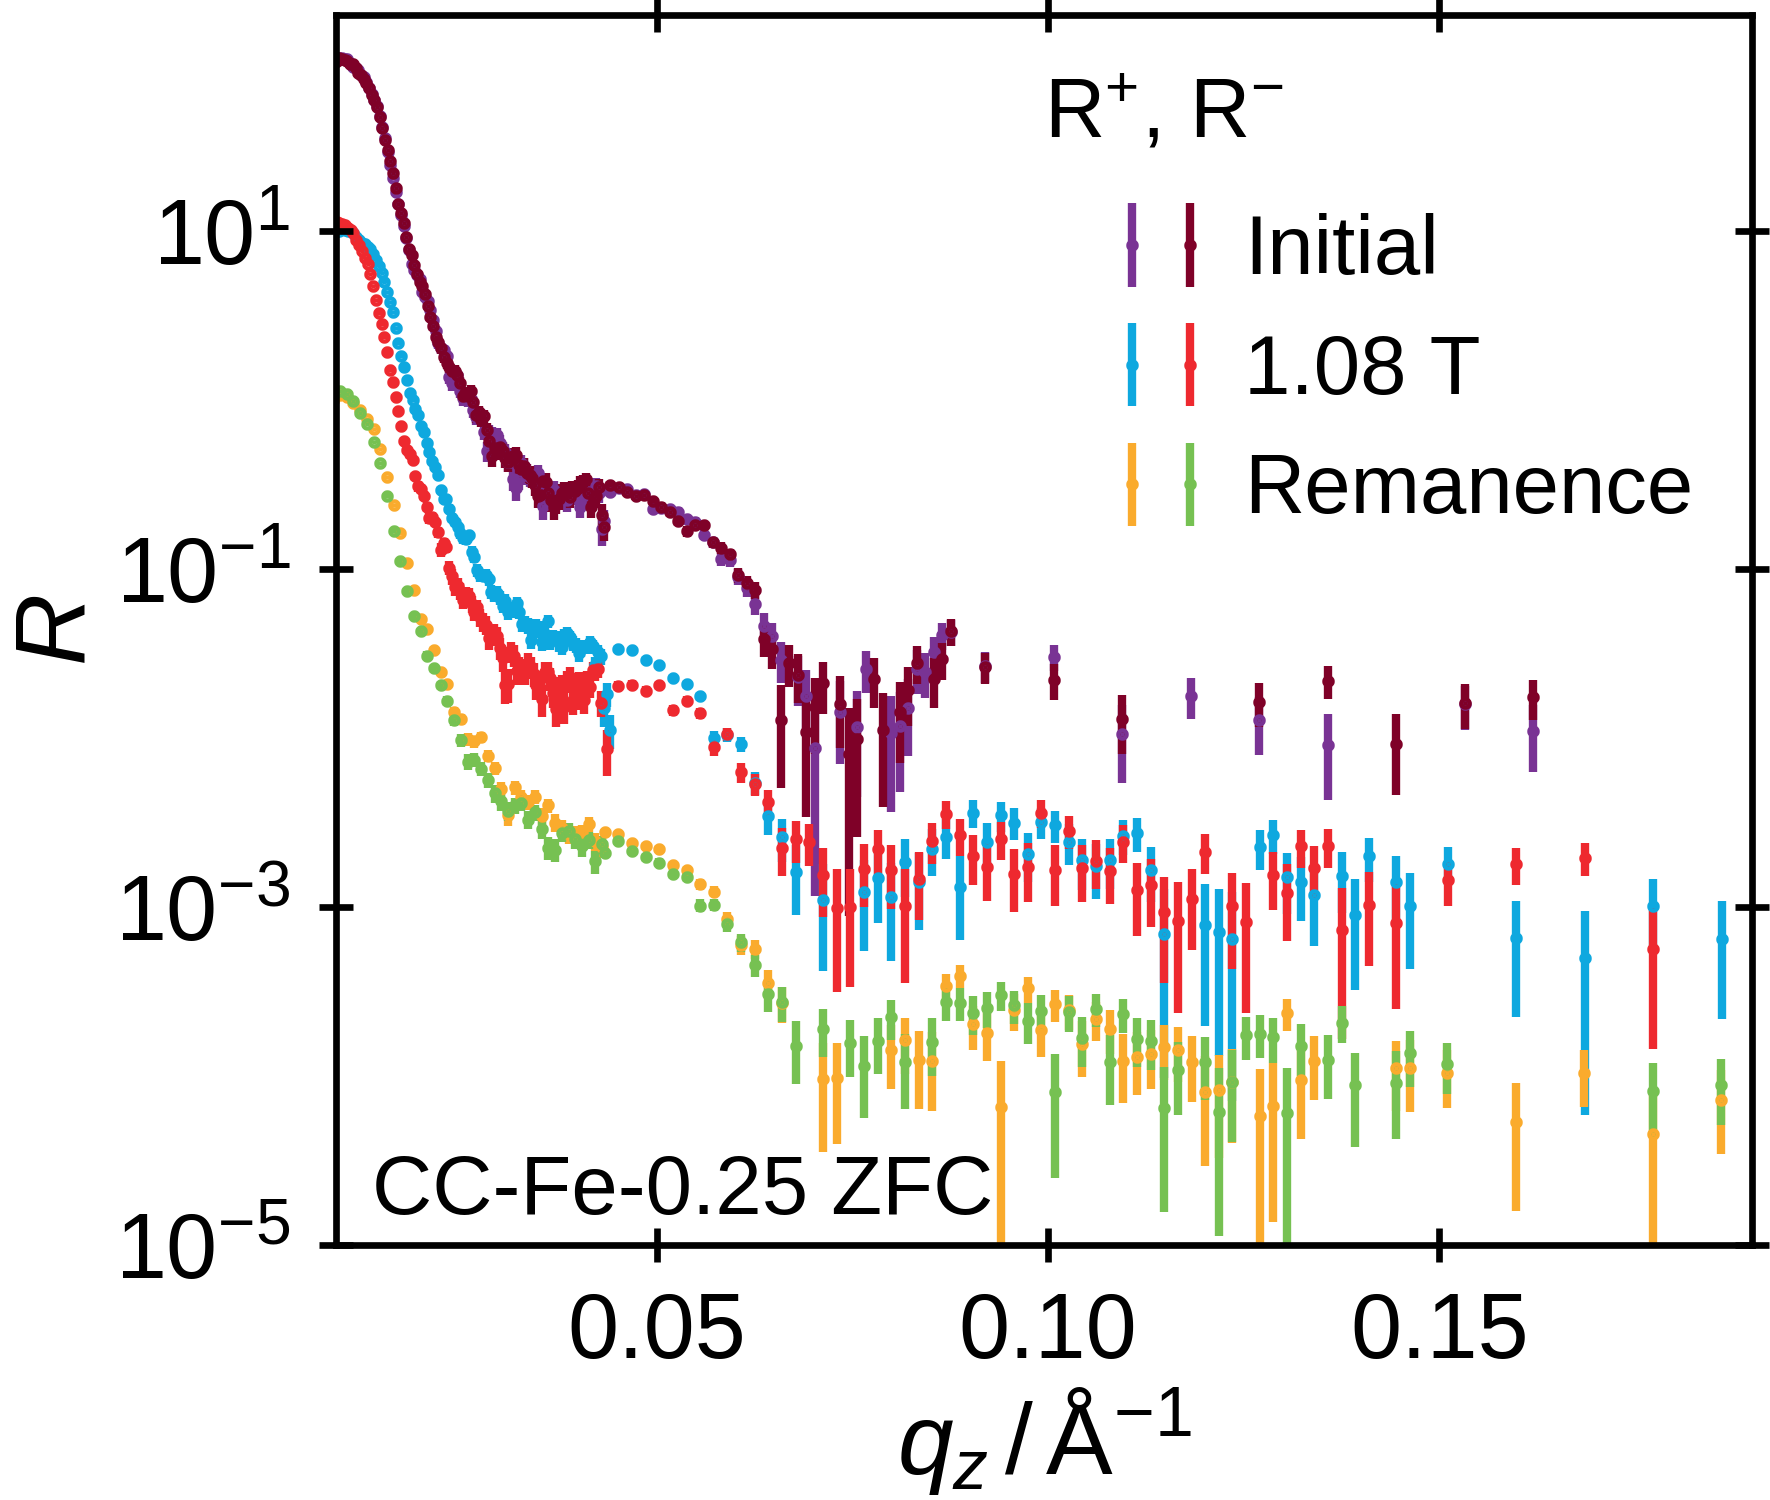
\includegraphics{colloidalCrystals_VerticalStructure_CC-Fe-0_25_PNR_ZFC10K}
    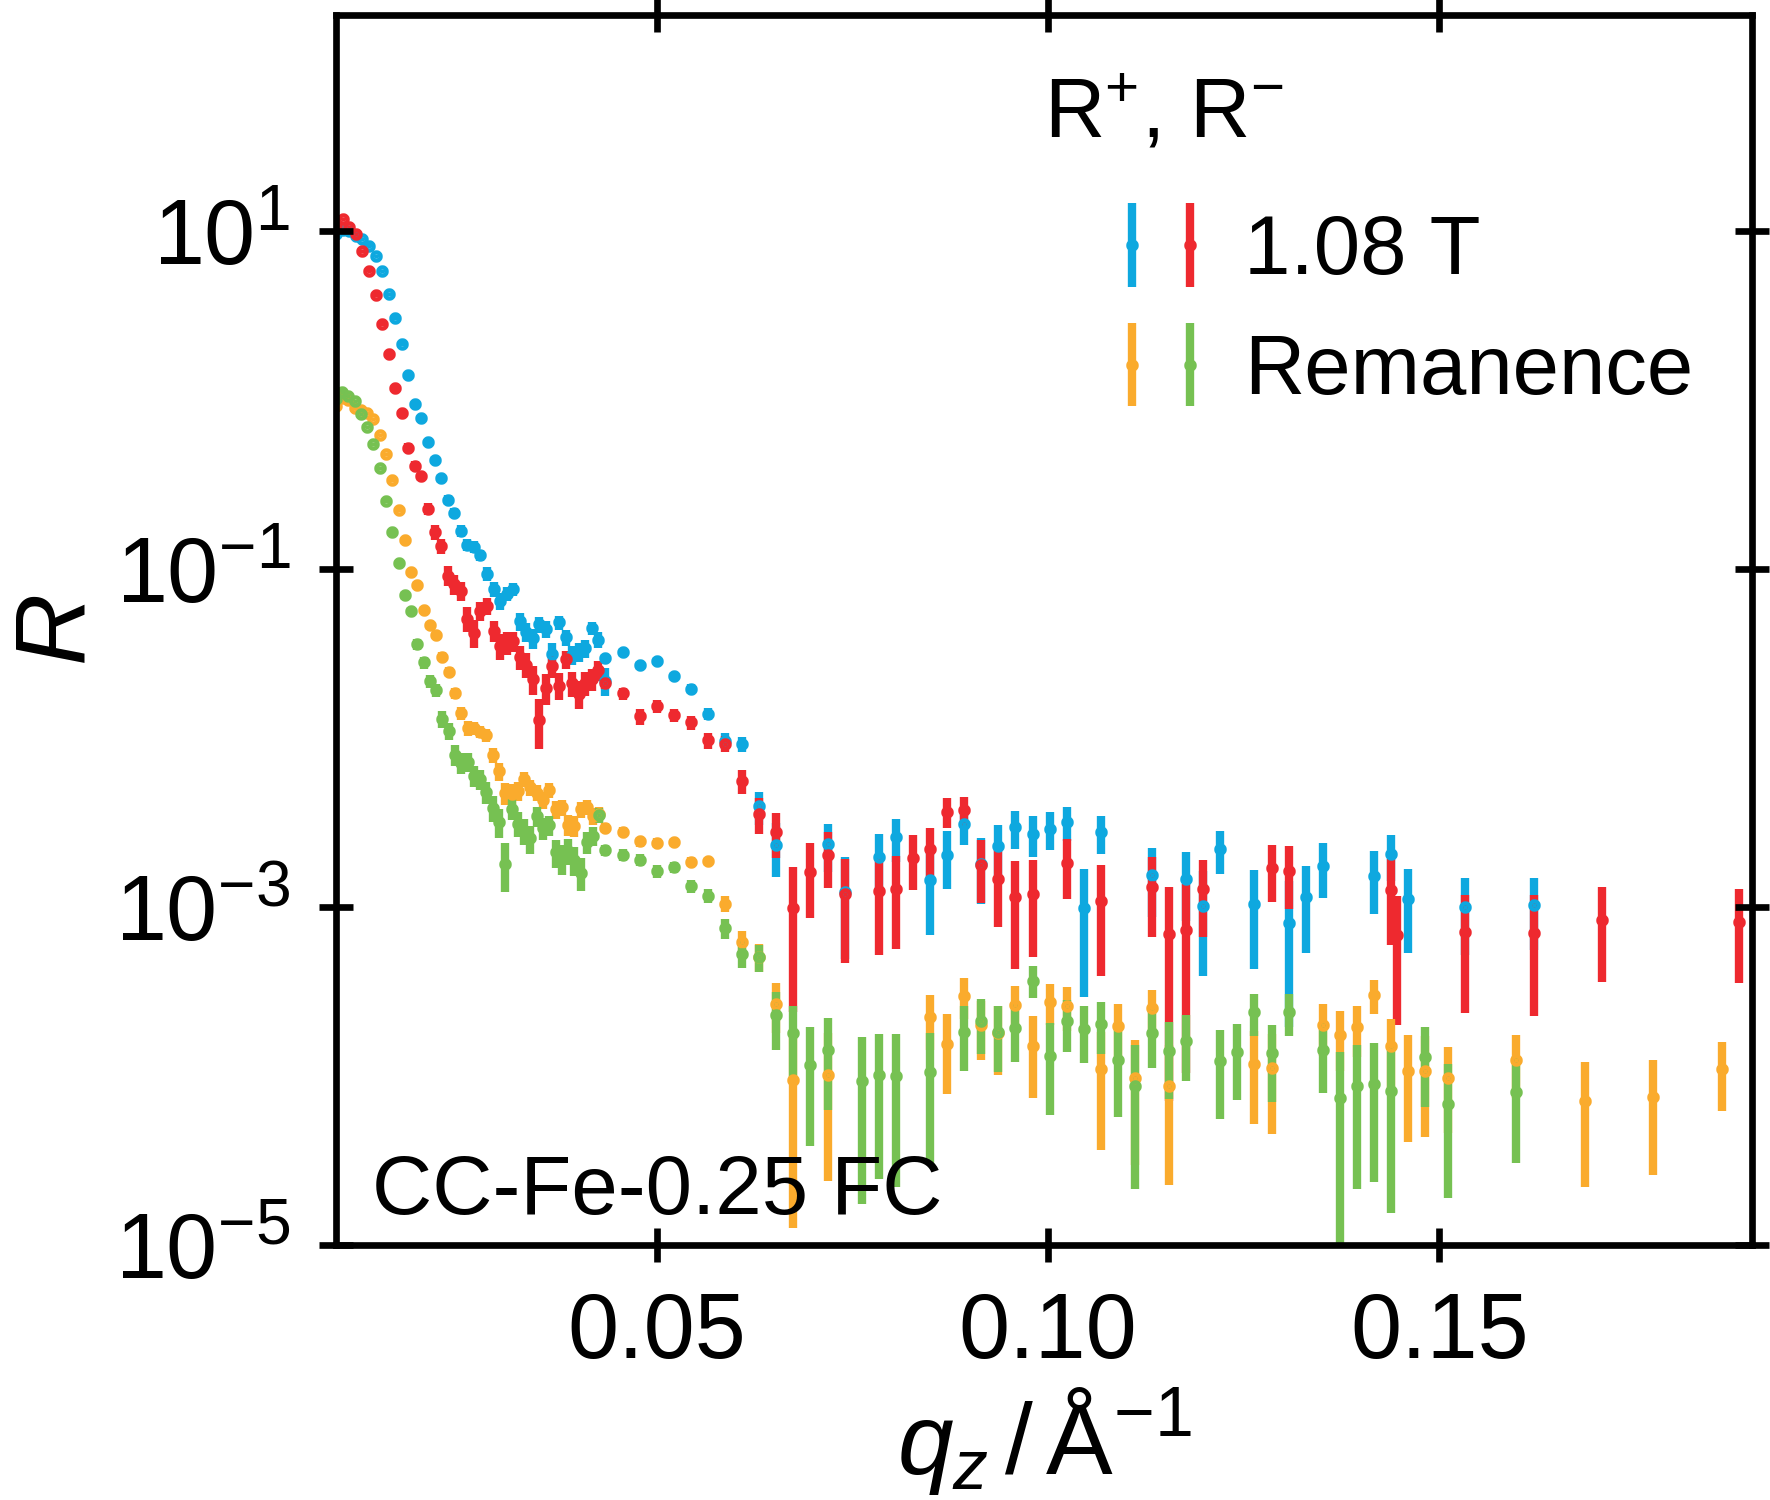
\includegraphics{colloidalCrystals_VerticalStructure_CC-Fe-0_25_PNR_FC10K}
    \caption{\label{fig:colloidalCrystals:pnr} CC-Fe-0.25 ZFC and FC}
  \end{figure}

  \begin{figure}[tb]
    \centering
    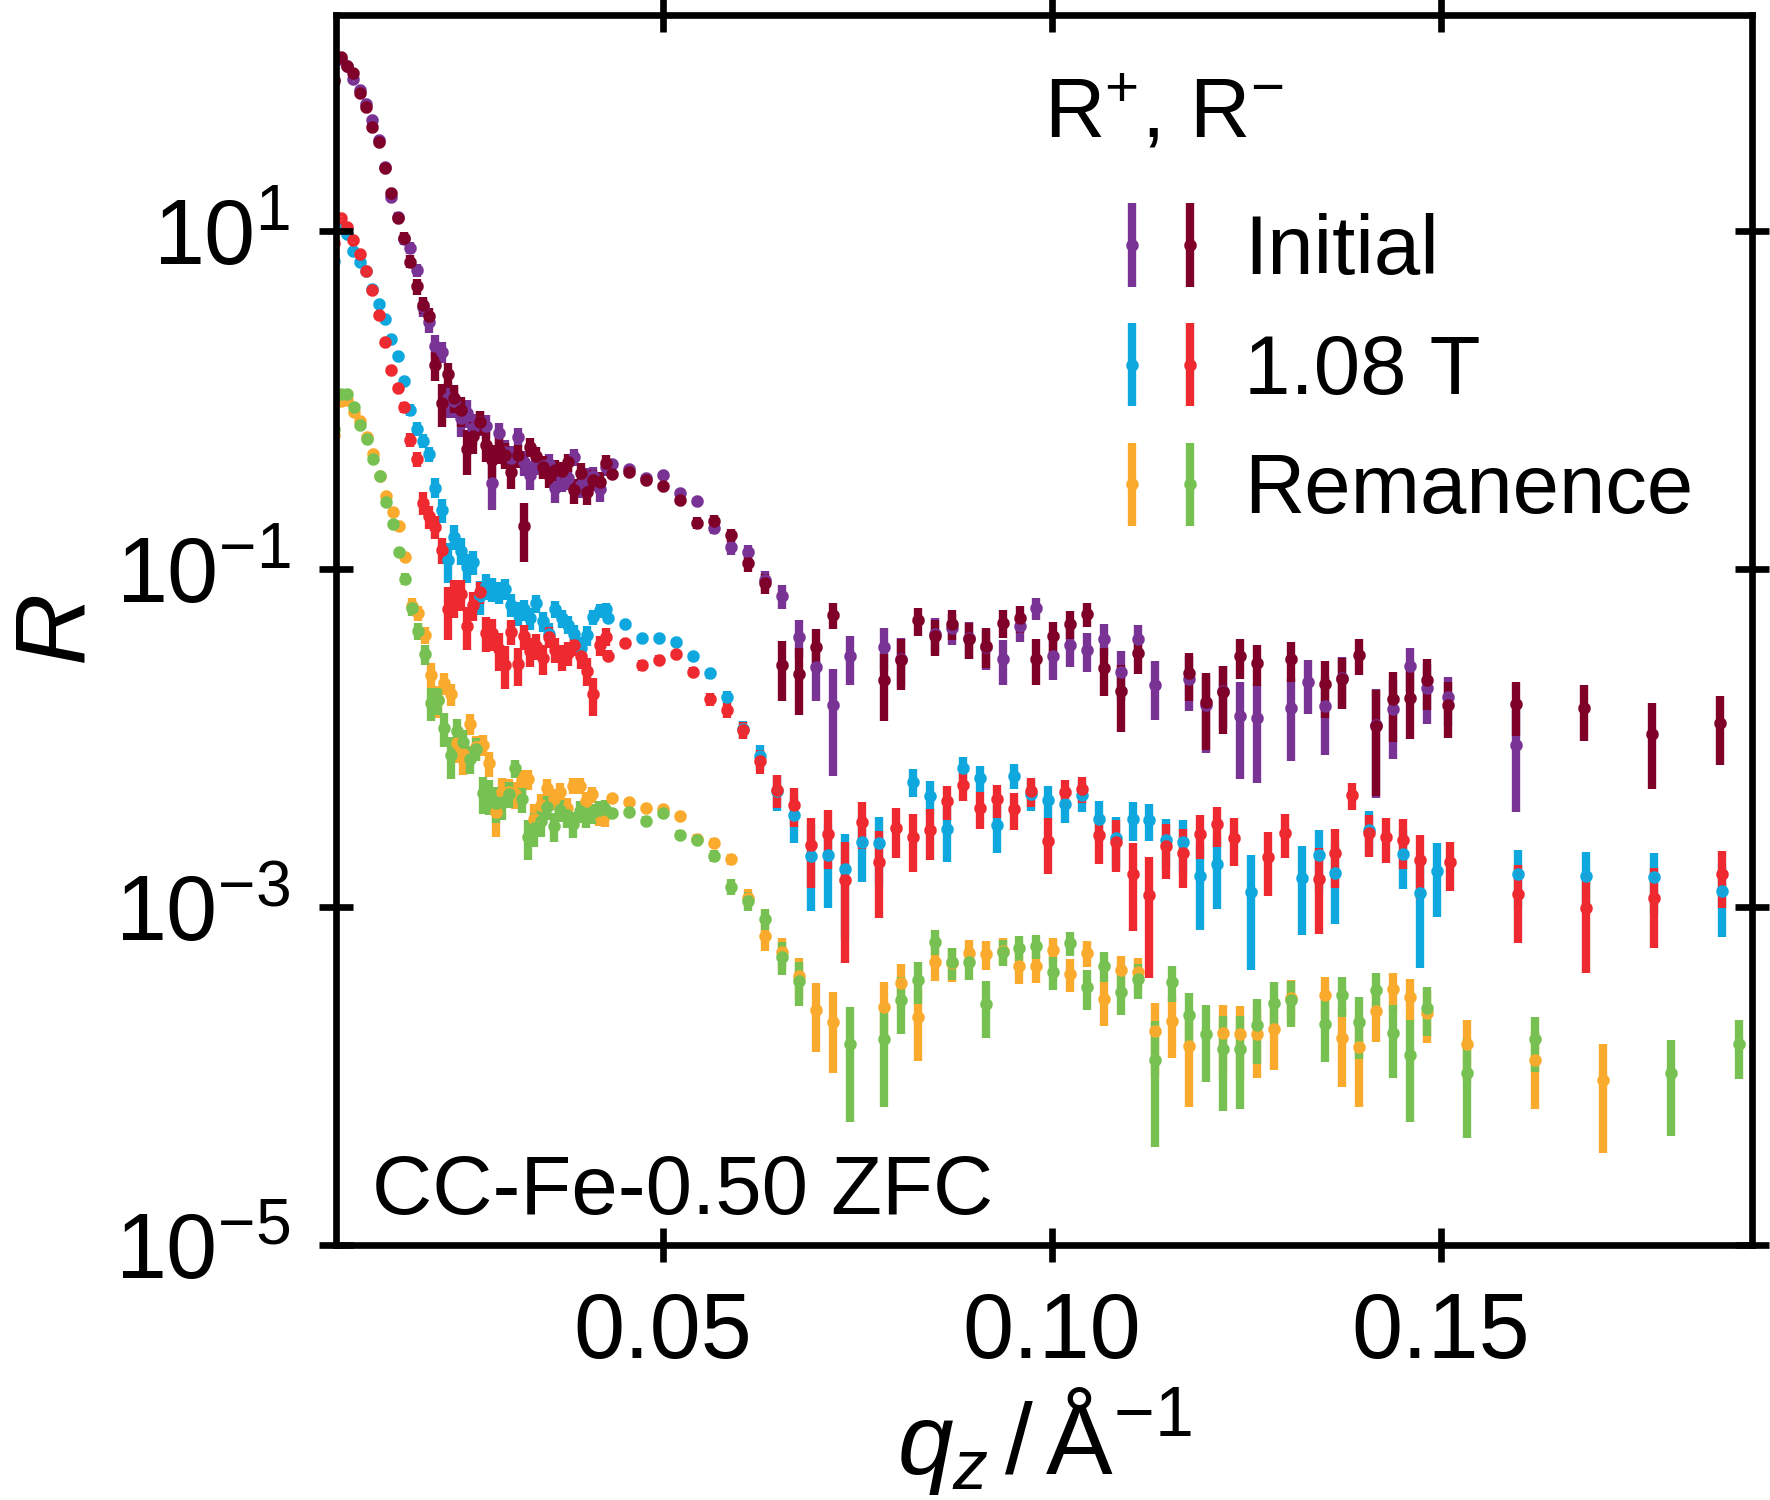
\includegraphics{colloidalCrystals_VerticalStructure_CC-Fe-0_50_PNR_ZFC10K}
    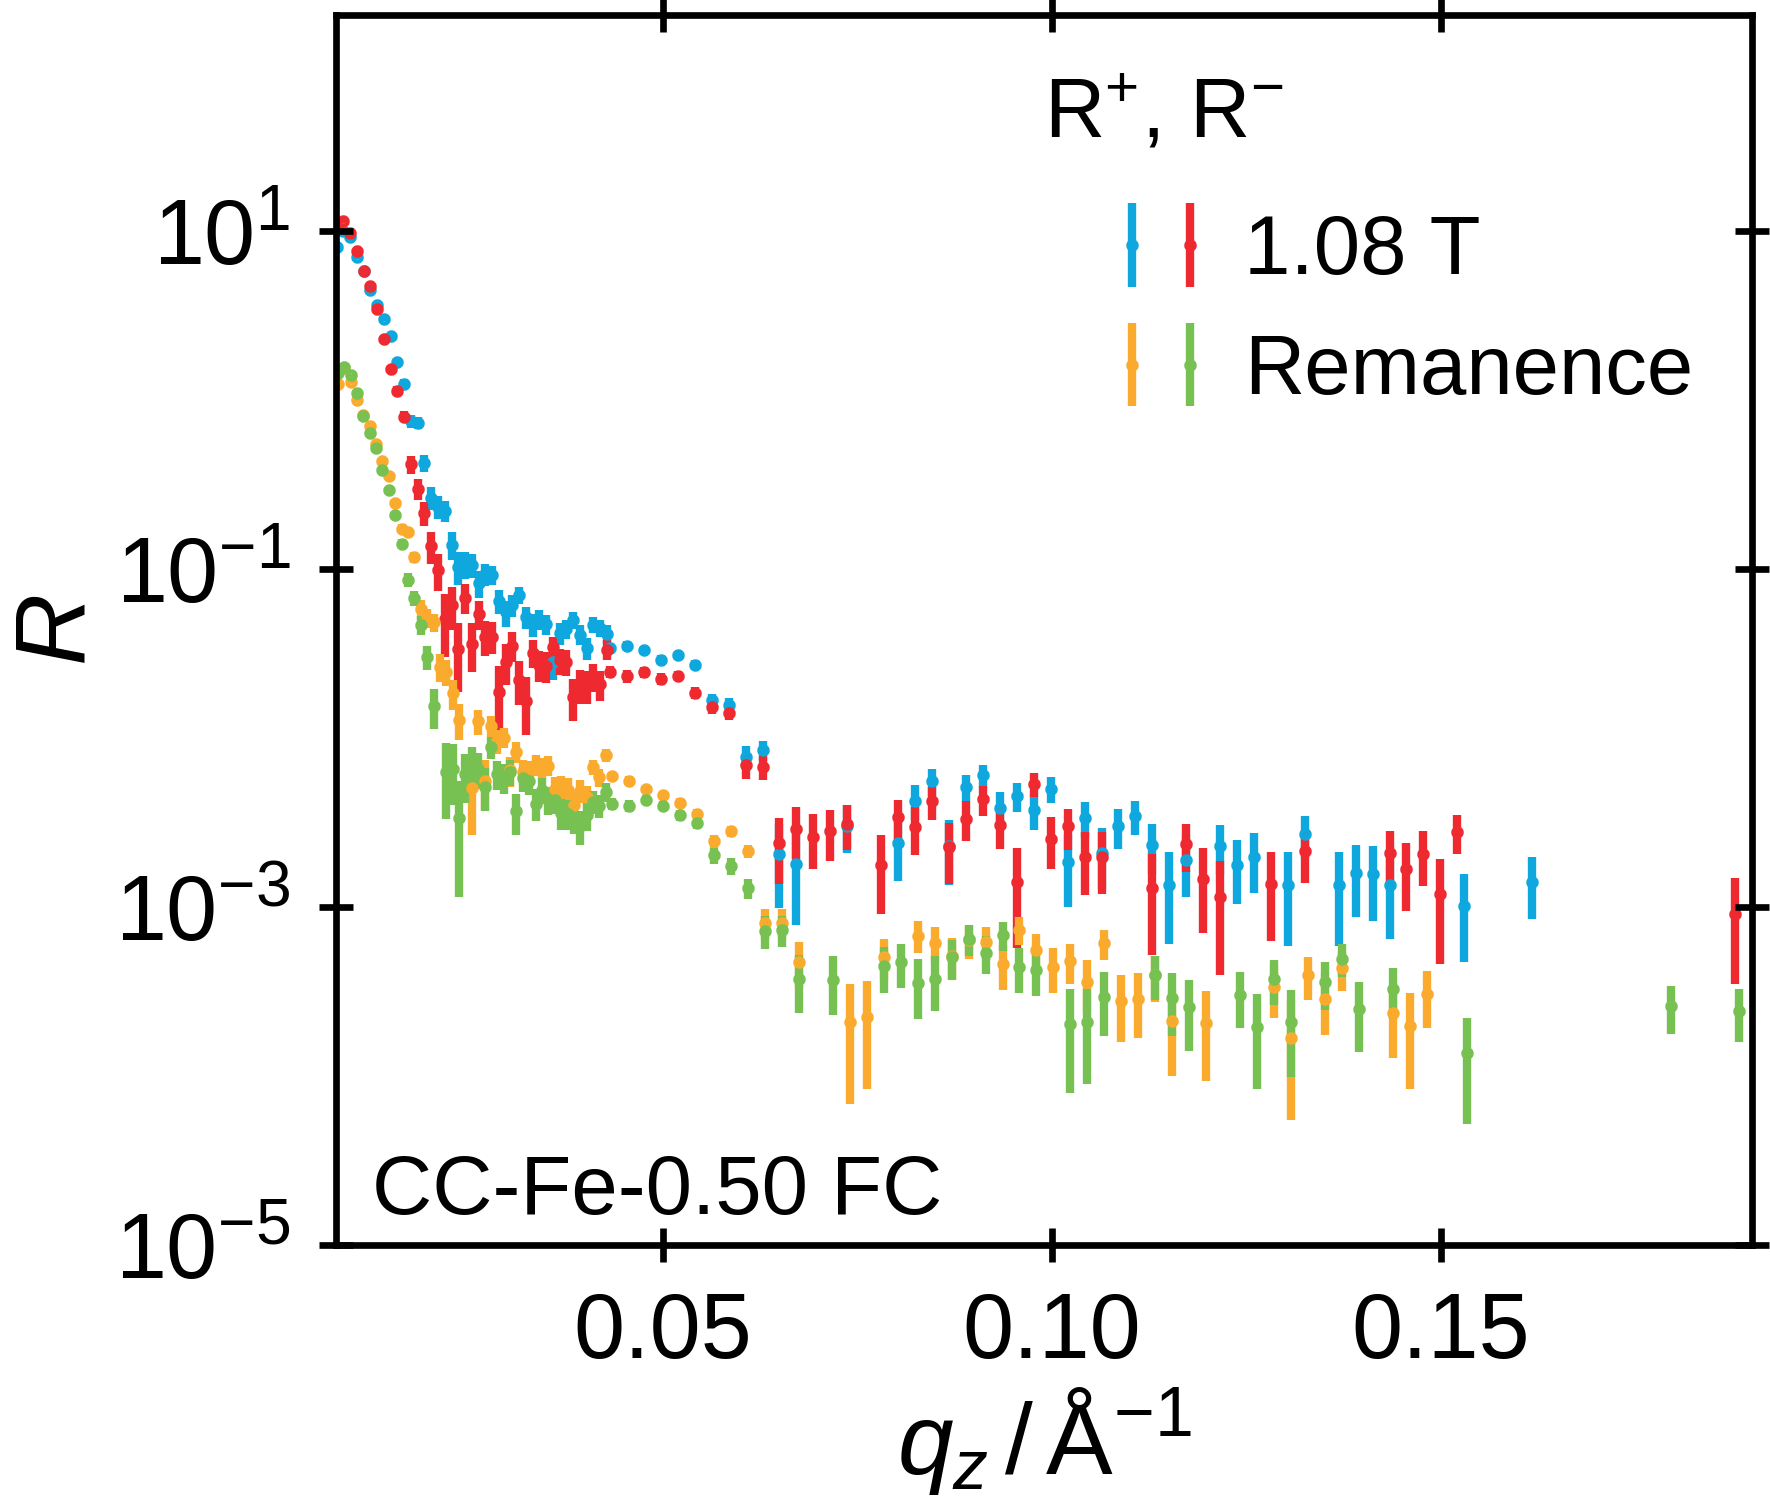
\includegraphics{colloidalCrystals_VerticalStructure_CC-Fe-0_50_PNR_FC10K}
    \caption{\label{fig:colloidalCrystals:pnr} CC-Fe-0.50 ZFC and FC}
  \end{figure}

\end{document}